\section{Results and Discussion} \label{sec:results}

\begin{figure}

\begin{subfigure}[c]{\linewidth} \centering
\begin{minipage}[c]{0.08\linewidth} \flushright
    \caption{\rotatebox[origin=c]{90}{25 cycles}}
    \label{fig:tagged_25}
  \end{minipage}%
  \begin{minipage}[c]{0.92\linewidth}
    \includegraphics[width=\textwidth,height=0.6in,trim={0 0.81cm 0 0},clip]{binder-wse-sketches/binder/teeplots/genome=hsurftiltedsticky_tagged+replicate=e4ea2071-8228-42de-af8c-879cedff9ba7+viz=draw-biopython-tree+ext=}
  \end{minipage}%
\end{subfigure}

\vspace{-1ex}

\begin{subfigure}[c]{\linewidth} \centering
\begin{minipage}[c]{0.08\linewidth} \flushright
    \caption{\rotatebox[origin=c]{90}{50 cycles}}
    \label{fig:tagged_50}
  \end{minipage}%
  \begin{minipage}[c]{0.92\linewidth}
    \includegraphics[width=\textwidth,height=0.6in,trim={0 0.81cm 0 0},clip]{binder-wse-sketches/binder/teeplots/genome=hsurftiltedsticky_tagged+replicate=3d55af5f-7714-45da-9276-e860f46b4d94+viz=draw-biopython-tree+ext=}
  \end{minipage}%
\end{subfigure}

\vspace{-1ex}

\begin{subfigure}[c]{\linewidth} \centering
  \begin{minipage}[c]{0.08\linewidth} \flushright
    \caption{\rotatebox[origin=c]{90}{100 cycles}}
    \label{fig:tagged_100}
  \end{minipage}%
  \begin{minipage}[c]{0.92\linewidth}
    \includegraphics[width=\textwidth,height=0.6in,trim={0 0.81cm 0 0},clip]{binder-wse-sketches/binder/teeplots/genome=hsurftiltedsticky_tagged+replicate=932aa302-becb-47e8-9712-7f550b02364c+viz=draw-biopython-tree+ext=}
  \end{minipage}%
\end{subfigure}

\vspace{-1ex}

\begin{subfigure}[c]{\linewidth} \centering
  \begin{minipage}[c]{0.08\linewidth} \flushright
    \caption{\rotatebox[origin=c]{90}{250 cycles}}
    \label{fig:tagged_250}
  \end{minipage}%
  \begin{minipage}[c]{0.92\linewidth}
    \includegraphics[width=\textwidth,height=0.8in]{binder-wse-sketches/binder/teeplots/genome=hsurftiltedsticky_tagged+replicate=42dbcbb3-b803-41a4-9285-4a450bfad6ed+viz=draw-biopython-tree+ext=}
  \end{minipage}%
\end{subfigure}

\caption{%
\textbf{Clade Validation Trial.}
\footnotesize
Example phylogenies reconstructed from runs of increasing duration on virtual grid of nine hardware-simulated PEs.
Founding genomes were tagged with random 16-byte identifier values, which were held constant over the course of simulation (Supplementary Figure \ref{fig:genome-layout}).
Color-coding indicates each sampled taxon's founding ancestor according to this identifier value.
Simulation performed under drift conditions.
}
\label{fig:tagged}

\end{figure}


\begin{figure*}
  \centering
  \includegraphics[width=\textwidth]{binder-reconstruction-quality/binder/surf-vs-col/outplots/surf-vs-col-table}
  \caption{%
    Column (red) vs. surface (blue) performance.
    For heatmap charts, +'s indicate small, medium, and large effect sizes using the Cliff's delta statistic and *'s indicate statistical significance at $\alpha = 0.05$ via Mann-Whitney U test.
  }
  \label{fig:col-vs-surf}
\end{figure*}


\subsection{Surface Algorithm Benchmark}

\begin{figure*}
  \centering
  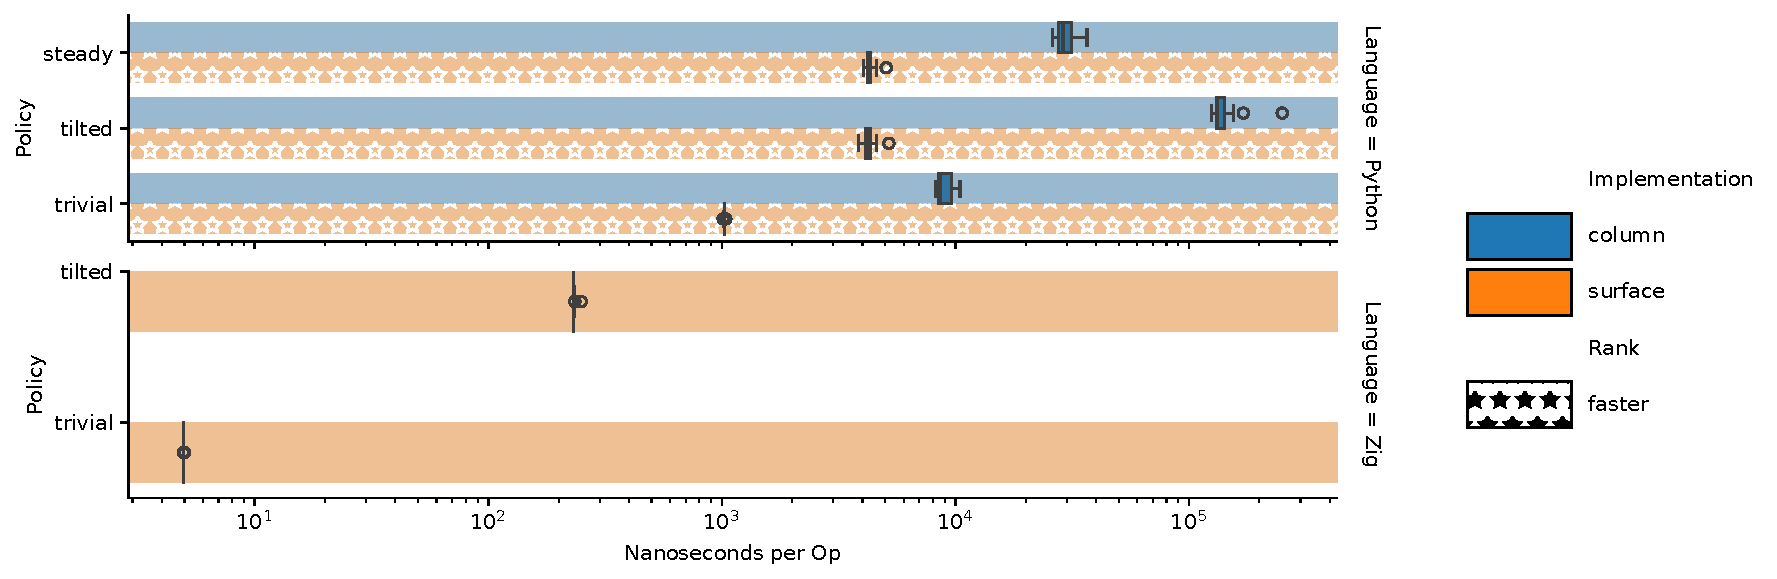
\includegraphics[width=0.85\textwidth,trim={0 0 0 0.4in
  }, clip]{binder-wafer-scale/binder/teeplots/all=false+hue=implementation+orient=h+row=language+score=nanoseconds-per-op+viz=peckplot+x=nanoseconds-per-op+y=policy+y-group=outer+ext=}

\vspace{-2.5ex}

  \caption{%
    \textbf{Hereditary stratigraphy algorithm benchmarks.}
    \footnotesize
    Comparison of per-generation operation time for column- and surface-based steady and tilted retention policies, lower is better.
  Top and bottom panels show Python and Zig implementations, respectively.
    Trivial is a simple harcoded retention decision, provided as a baseline control.
    Background hatching indicates significant outcome (Mann-Whitney U test; $n=20$).
  }
  \label{fig:benchmarking}
  \vspace{-0.2in}
\end{figure*}


We performed benchmarking experiments to assess the computational performance of our new surface-based algorithms.
Due to limited completed implementations of compiled-language algorithms, we performed the bulk of benchmarking using the Python implementations.
While Python is an interpreted language and the Python-implemented algorithms weren't specifically implemented to maximize performance, and has an intrinsic performance penalty due to that, the algorithms were all in the same footing and we use the ``optimize''' flag to strip assert statements out of the benchmarks.
However, in the process of porting the tilted surface algorithm over to Cerebras Software Language we did create an implementation of that algorithm in Zig which is a compiled language and is capable of compiler optimizations.
We augment the Python with a benchmark of this algorithm.
Figure \ref{fig:benchmarking} provides an overview of results.

% https://github.com/mmore500/hstrat-surface-concept/blob/51d636d768d474fc5148b9fcaa199c1b7776e915/benchmark.ipynb
We found that the Python implementations of the surface tilted and steady algorithms both took around 4,200ns per operation (SEM c. 50; $n=20$).
For context, this was about $4\times$ the measured time for a surface placement using a trivial calculation (SEM c. 0.05; $n=20$).
The column implementations of steady and tilted fared much worse, taking about $7\times$ and $34\times$ the execution time per operation compared to the surface operations.
Mann-Whitney U tests confirmed that surface implemnetations significantly outperformed their column counterparts. (Figure \ref{fig:benchmarking}).

% https://github.com/mmore500/wse-sketches/blob/d4ab0155f63ff5809f8eeca1169ad9b272c30a68/binder/benchmark.ipynb
Zig implementation of tilted surface:
233 ns per operation (SEM 0.9; $n=20$).
This was $47\times$ the measured time for a trivial placement calculation (SEM 0.2; $n=20$).
For context, this time a little more than twice the amount of time required for a main memory access in contemporary computing hardware \citep{markus2022memory}.

Note that further speedups and optimizations can likely to be had.
For single-bit differentiae, half of the time placement need not be calculated if the coin flip indicates that the bit isn't going to be flipped.
Further, in synchronous and near-synchronous simulations, placement positions can be cached meaning they would only need to be calculated once for an entire subpopulation.

\subsection{WSE Genetic Algorithm Benchmark}

We used the cycle counter on the WSE hardware simulator to test the amount of real time elapsed over the course of a 100 generation cycle simulation on a $3\times3$ PE collective with the tagged 3 word genome, applying a tilted hereditary stratigraphy every generation.

Each PE completed a mean 29,500 generation cycles per second (SEM 155; $n=9$), or around 2 billion generations a day.
Over the course of the simulation each PE immigrated a mean of 277 genomes (SEM 23; $n=9$).

How would this look on a full piece of hardware?
Keeping 32 individuals per PE would result in a net population size of around 27 million on a full WSE.
(Although generation time would be slower, available memory on the CS-2 could support on the order of thousands of agents per PE potentially yielding a net population size on the order of a billion agents.)
% 29,500 * 850,000 * 60 * 60 * 24 * 32 ---> 69 quadrillion
Naive extrapolation would estimate on the order of a quadrillion agent replications every half hour, notwithstanding scaling slowdown.

% https://github.com/mmore500/wse-sketches-mirror/actions/runs/8546407499/job/23416697013
% from https://github.com/mmore500/wse-sketches-mirror/commit/fb7f9c4e175818253f844909297d747cd813b9c7
% Reading file out/out.json
% Reading file out/bin/out_rpc.json
% Reading file out/west/out.json
% Reading file out/east/out.json
% fab w,h = 10,5
% Kernel x,y w,h = 4,1 3,3
% memcpy x,y w,h = 1,1 8,3
% ASYNC_GA_GLOBAL_SEED 3
% ASYNC_GA_NCYCLE 100
% CSLC cslc
% ASYNC_GA_GENOME_FLAVOR genome_hsurftiltedsticky_tagged
% ASYNC_GA_GLOBAL_SEED 3
% ASYNC_GA_NCYCLE 100
% INFO: Using SIF: /home/runner/cerebras/bin/cbcore_sdk-202311111408-10-4a54bce5.sif
% INFO: User's specified CSL_IMPORT_PATH=
% NOTE: CSL_IMPORT_PATH accepts colon separated list of paths generated by 'realpath <path>'
% INFO:    Environment variable SINGULARITYENV_CSL_SUPPRESS_SIMFAB_TRACE is set, but APPTAINERENV_CSL_SUPPRESS_SIMFAB_TRACE is preferred
% compile successful
% Updated 1 path from the index
% CS_PYTHON cs_python
% INFO: Using SIF: /home/runner/cerebras/bin/cbcore_sdk-202311111408-10-4a54bce5.sif
% INFO:    Environment variable SINGULARITYENV_CSL_SUPPRESS_SIMFAB_TRACE is set, but APPTAINERENV_CSL_SUPPRESS_SIMFAB_TRACE is preferred
% whoami ===============================================================
% [[0 3 6]
%  [1 4 7]
%  [2 5 8]]
% whereami x ===========================================================
% [[0 1 2]
%  [0 1 2]
%  [0 1 2]]
% whereami y ===========================================================
% [[0 0 0]
%  [1 1 1]
%  [2 2 2]]
% cycle counter =======================================================
% [[100 100 100]
%  [100 100 100]
%  [100 100 100]]
% recv counter N ========================================================
% [[ 1  1  1]
%  [29 25 29]
%  [27 25 26]]
% recv counter S ========================================================
% [[23 25 25]
%  [25 27 23]
%  [ 1  1  1]]
% recv counter E ========================================================
% [[25 29  1]
%  [25 26  1]
%  [23 27  1]]
% recv counter W ========================================================
% [[ 1 23 24]
%  [ 1 23 25]
%  [ 1 25 27]]
% recv counter sum =====================================================
% [50, 78, 51, 80, 101, 78, 52, 78, 55]
% np.mean(recvSum)=69.22222222222223 np.std(recvSum)=16.857426835260856 sps.sem(recvSum)=5.960000414284516
% send counter N ========================================================
% [[100 100 100]
%  [100 100 100]
%  [100 100 100]]
% send counter S ========================================================
% [[112 102 112]
%  [108 100 104]
%  [  0   0   0]]
% send counter E ========================================================
% [[ 90 100   0]
%  [ 94 102   0]
%  [102 110   0]]
% send counter W ========================================================
% [[  0 102 112]
%  [  0 100 104]
%  [  0  92 108]]
% send counter sum =====================================================
% [202, 304, 224, 296, 404, 306, 204, 312, 202]
% np.mean(sendSum)=272.6666666666667 np.std(sendSum)=65.40812046085885 sps.sem(sendSum)=23.125262761269934
% tscControl values ====================================================
% [30064968187, 30064968187, 30064968187, 30064968187, 30064968187, 30064968187, 30064968187, 30064968187, 30064968187]
% tscStart values ======================================================
% [2623, 2137, 1653, 3133, 2648, 2114, 1627, 3111, 3111]
% tscEnd values ========================================================
% [2833350, 2958017, 2834797, 2901552, 2894748, 2906881, 2847462, 2935863, 2847357]
% tsc diffs ============================================================
% --------------------------------------------------------------- ticks
% [2830727, 2955880, 2833144, 2898419, 2892100, 2904767, 2845835, 2932752, 2844246]
% np.mean(tsc_ticks)=2881985.5555555555 np.std(tsc_ticks)=43041.3869074125 sps.sem(tsc_ticks)=15217.428276952633
% -------------------------------------------------------------- seconds
% [0.0033302670588235294, 0.0034775058823529412, 0.003333110588235294, 0.003409904705882353, 0.003402470588235294, 0.0034173729411764706, 0.003348041176470588, 0.0034502964705882353, 0.003346171764705882]
% np.mean(tsc_sec)=0.0033905712418300657 np.std(tsc_sec)=5.0636925773426534e-05 sps.sem(tsc_sec)=1.7902856796414882e-05
% ---------------------------------------------------- seconds per cycle
% [3.330267058823529e-05, 3.477505882352941e-05, 3.333110588235294e-05, 3.409904705882353e-05, 3.402470588235294e-05, 3.4173729411764705e-05, 3.348041176470588e-05, 3.4502964705882353e-05, 3.346171764705882e-05]
% np.mean(tsc_cysec)=3.390571241830066e-05 np.std(tsc_cysec)=5.063692577342663e-07 sps.sem(tsc_cysec)=1.7902856796414917e-07
% ---------------------------------------------------------- cycle hertz
% [30027.621879467715, 28756.241796013368, 30002.00483985283, 29326.332735191147, 29390.408353791365, 29262.243753113416, 29868.210911735925, 28983.016634205687, 29884.897438547865]
% np.mean(tsc_cyhz)=29500.1087046577 np.std(tsc_cyhz)=438.84515891452514 sps.sem(tsc_cyhz)=155.15519387967439
% --------------------------------------------------------- ns per cycle
% [33302.67058823529, 34775.05882352941, 33331.10588235294, 34099.04705882353, 34024.70588235294, 34173.7294117647, 33480.41176470588, 34502.964705882354, 33461.717647058824]
% np.mean(tsc_cyns)=33905.71241830065 np.std(tsc_cyns)=506.36925773426583 sps.sem(tsc_cyns)=179.028567964149
% genome values ========================================================
% ------------------------------------------------ genome binary strings
% 110101001011011001011001000000001110100101011110101001110010101000110100110101111010000000000100
% 000001111101100101011000000000001111110001111111110001100000101111101011110011001100110110110010
% 110110011001011101011101000000001010011011101000100100110001110110010000100010100111001111000101
% 001110001101110101011100000000001000110110011100000010010011100010010011110001101001011100001110
% 001110001101110101011011000000001000110100000100100000110001100000010010100000101001011100001100
% 000001111101100101100000000000001111110000100110110001111111000011110010010111101111001100100101
% 001110001101110101011011000000001100111100010101010000110011000011110110000100111011010001000101
% 000001111101100101010101000000001011110001011101100000000101010111110101110101000111010001001001
% 100110001100100101001111000000001000100110101110011111111000010001011101000001000110010001011110
% --------------------------------------------------- genome hex strings
% D4B65900E95EA72A34D7A004
% 07D95800FC7FC60BEBCCCDB2
% D9975D00A6E8931D908A73C5
% 38DD5C008D9C093893C6970E
% 38DD5B008D0483181282970C
% 07D96000FC26C7F0F25EF325
% 38DD5B00CF154330F613B445
% 07D95500BC5D8055F5D47449
% 98C94F0089AE7F845D04645E
% SUCCESS!
% Reading file out/out.json
% Reading file out/bin/out_rpc.json
% Reading file out/west/out.json
% Reading file out/east/out.json
% fab w,h = 10,5
% Kernel x,y w,h = 4,1 3,3
% memcpy x,y w,h = 1,1 8,3

\subsection{On-hardware Demonstration with Evolutionary Inference from Phylogenetic Analysis}

\begin{figure*}
  \centering
  \begin{minipage}{\textwidth}
    \centering
    Generations Ago (approx.)
  \end{minipage}
  \begin{minipage}{\textwidth}
    \hspace{0.02\linewidth}
    \rotatebox{30}{\makebox[0.1\linewidth][c]{200,000}}
    \hfill
    \rotatebox{30}{\makebox[0.1\linewidth][c]{50,000}}
    \hfill
    \rotatebox{30}{\makebox[0.1\linewidth][c]{10,000}}
    \hfill
    \rotatebox{30}{\makebox[0.1\linewidth][c]{2,000}}
    \hfill
    \rotatebox{30}{\makebox[0.1\linewidth][c]{30}}
    \rotatebox{90}{\makebox[0.04\linewidth][c]{0}}
  \end{minipage}
  \begin{subfigure}[t]{\linewidth}
    \centering
  \includegraphics[width=\linewidth,height=0.3\linewidth]{bindertex-evolutionary-inference/img/perfect-tree-phylogenies-log/epoch=7+resolution=3+treatment=22/a=collapsed-phylogeny+epoch=00007+mut_distn=np.random.standard_normal+num_generations=32768+num_islands=1024+num_niches=4+p_island_migration=0.01+p_niche_invasion=3.0517578125e-08+population_size=3276.../8+replicate=0+tournament_size=2+treatment=22+_generation=262144+_index=22+scale=log+ext=}
    \caption{%
    Tournament size 2.
    STAND-IN IMAGE.
    }
    \label{fig:wse-phylogenies-tsize2}
  \end{subfigure}

  \begin{subfigure}[t]{\linewidth}
    \centering
\includegraphics[width=\linewidth,height=0.3\linewidth]{bindertex-evolutionary-inference/img/perfect-tree-phylogenies-log/epoch=7+resolution=3+treatment=6/a=collapsed-phylogeny+epoch=00007+mut_distn=np.random.standard_normal+num_generations=32768+num_islands=1024+num_niches=1+p_island_migration=0.01+p_niche_invasion=3.0517578125e-08+population_size=3276.../8+replicate=0+tournament_size=2+treatment=6+_generation=262144+_index=6+scale=log+ext=}
    \caption{%
      Tournament size 8.
      STAND-IN IMAGE.
    }
    \label{fig:wse-phylogenies-tsize8}
  \end{subfigure}

\caption{%
\textbf{Phylogenies from on-hardware experiment.}
Subfigures \ref{fig:wse-phylogenies-tsize2} and \ref{fig:wse-phylogenies-tsize8} contrast phylogenies from experiments with lower and higher selection pressure, respectively.
Note the recognizable decrease in phylogenetic richness under high selection pressure.
Each phylogeny subsampled to 131,072 taxa.
}
\label{fig:wse-phylogenies}

\end{figure*}


In order to perform a preliminary assessment of the practicability of this methodology in practice, we ran our genetic algorithm on a WSE device.
We annotated genomes with a 64-bit instrumentative annotation, comprising a 32-bit counter and 32 bit tilted hstrat surface.
We performed evolutionary runs under two conditions, one with tournament size 2 and one with tournament size 8.
We performed TODO replicates per condition, running each for Y minutes.
This was sufficient to observe a mean of TODO generations per cycle, SD TODO.
At the conclusion of the run, we collected one genome from each PE.

Figure \ref{fig:wse-phylogenies} compares two example reconstructed phylogenies, one from each treatment.
Performing a reconstruction with all 850,000 genomes took X minutes.
We used a Mann-Whitney U test between inner node time distributions for pairs of trees to test whether the difference in selection pressure was detectable.
Indeed, the recovered phylogenetic information was sufficient to detect this difference in evolutionary dynamics for all pairs ($p < TODO$ for all $n=TODO$).
